\setcounter{section}{1}
\appendix
\clearpage{\renewcommand{\appendixname}{Anexo}

\chapter{Interfaz de usuario del sistema}

\section{Gestión de procesos}
\section{Entrenamiento de un proceso}
\subsection{Tipos de preguntas en la etapa de las variables}
\subsection{Tipos de preguntas en la etapa de las causas}
\subsection{Tipos de preguntas en la etapa de las recomendaciones}
\subsection{Resultados de una etapa}

\chapter{Pruebas funcionales del sistema}

\section{Insertar configuración de entrenamiento}
\begin{figure}[H]
\centering
 \frame{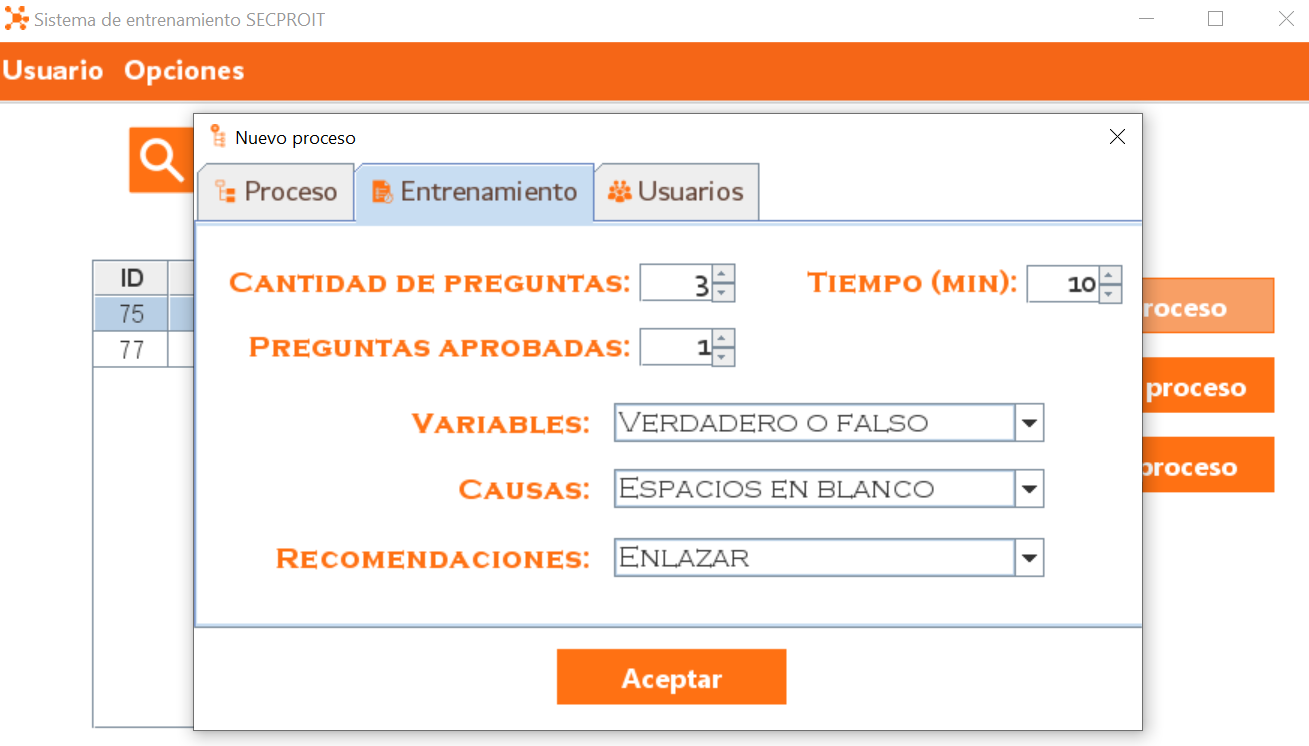
\includegraphics[width=0.9\linewidth]{imagen/anexos/nuevaConf.png}}
 \caption{Insertar configuración con campos en blanco}
 \label{fig:cb} 
\end{figure}

\begin{figure}[H]
\centering
 \frame{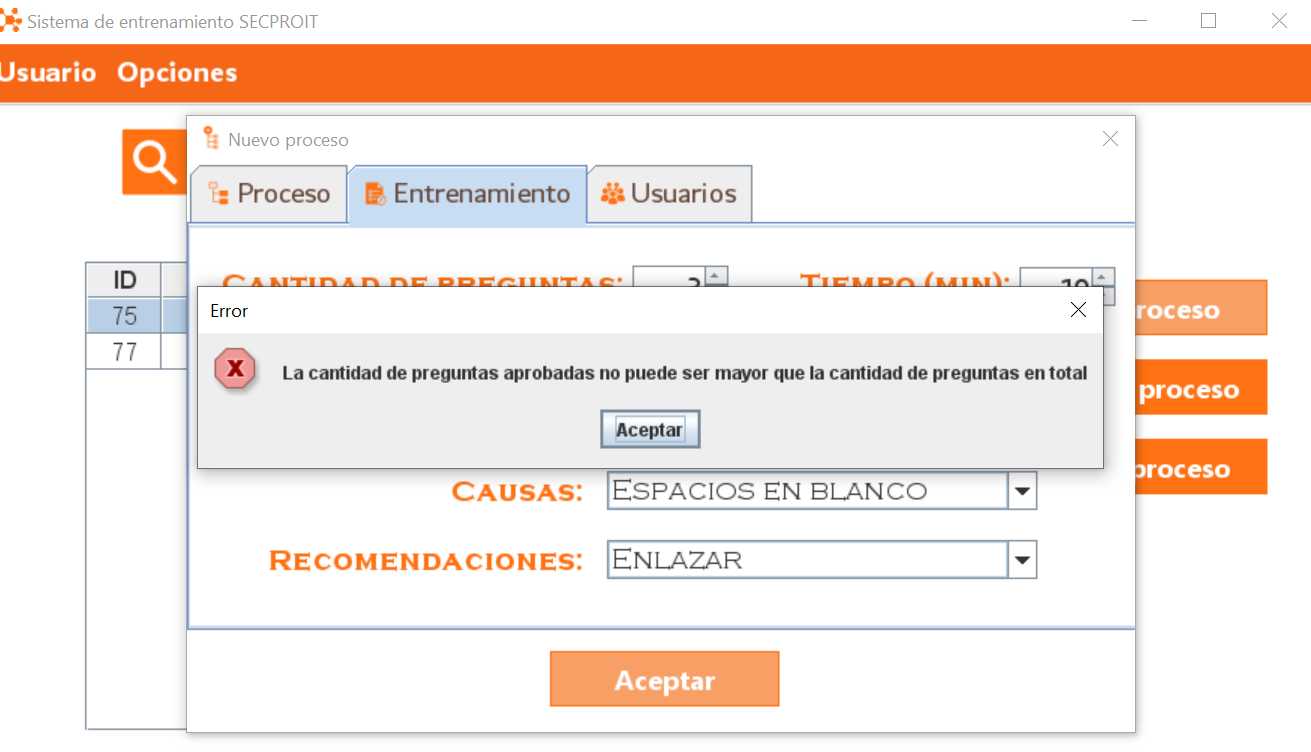
\includegraphics[width=0.9\linewidth]{imagen/anexos/errorConf.png}}
 \caption{Insertar configuración con campos incorrectos}
 \label{fig:ci} 
\end{figure}

\begin{figure}[H]
\centering
 \frame{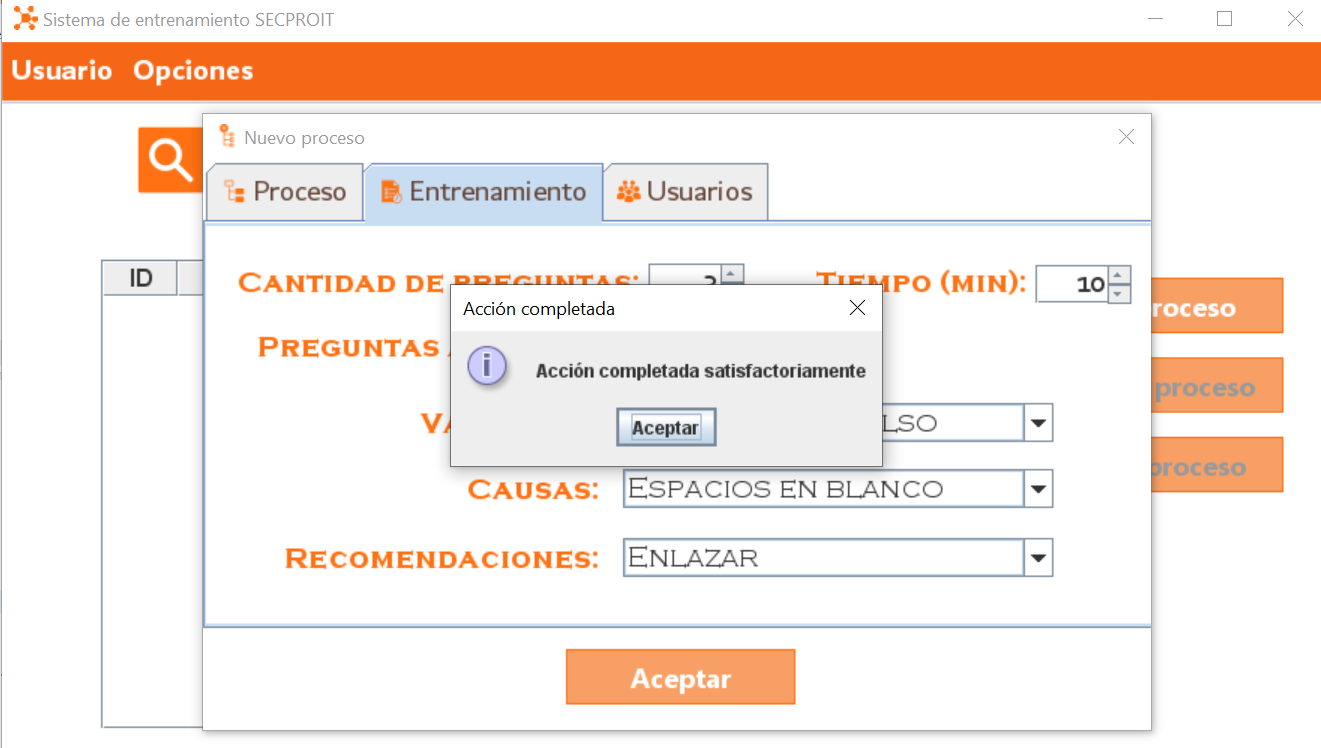
\includegraphics[width=0.9\linewidth]{imagen/anexos/guardarConf.png}}
 \caption{Insertar configuración con campos correctos}
 \label{fig:cc} 
\end{figure}

\section{Eliminar configuración de entrenamiento}
\begin{figure}[H]
\centering
 \frame{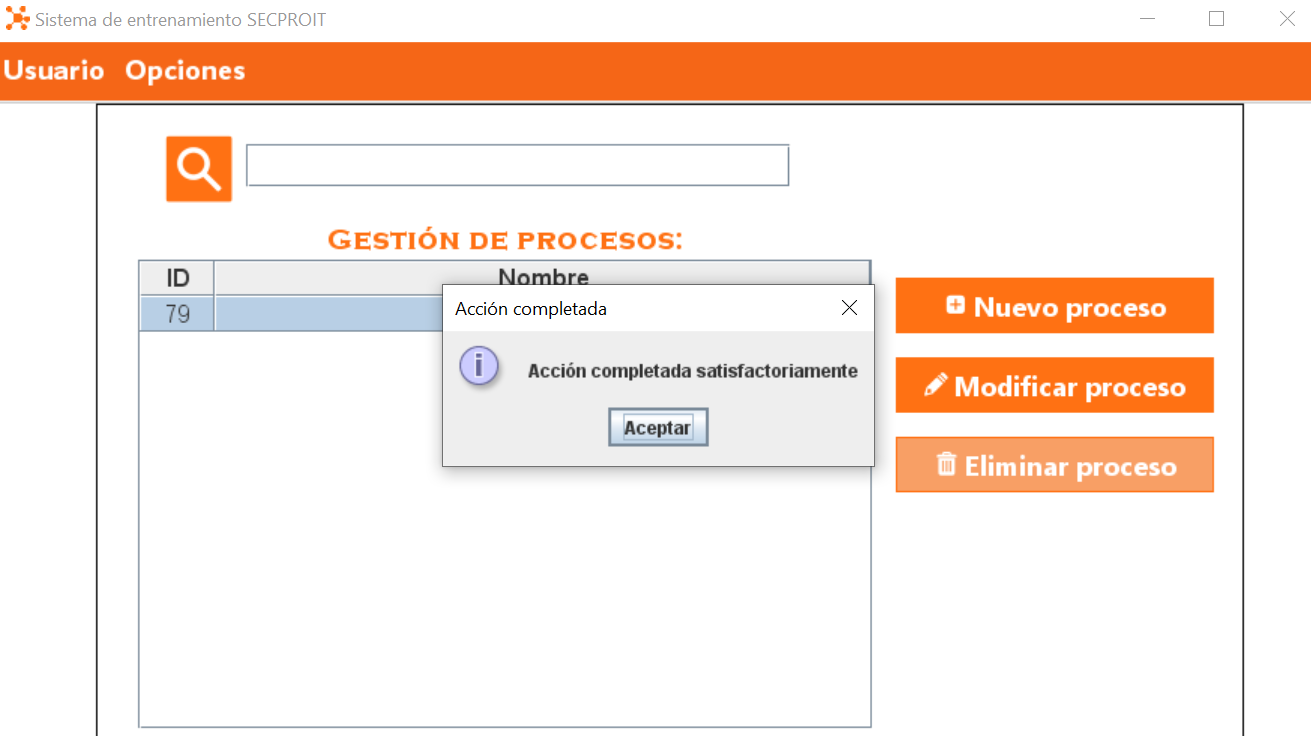
\includegraphics[width=0.9\linewidth]{imagen/anexos/eliminarConf.png}}
 \caption{Eliminar configuración de entrenamiento}
 \label{fig:ce} 
\end{figure}